\documentclass[11pt,a4paper]{article}
\usepackage[margin=21mm]{geometry}
\usepackage[T1]{fontenc}
\usepackage{lmodern,microtype,booktabs,graphicx,titlesec,multirow}
\usepackage[font=small,labelfont=bf]{caption}
\usepackage[hidelinks]{hyperref}
\setlength{\parindent}{0pt}
\setlength{\parskip}{4pt}
\titlespacing*{\section}{0pt}{9pt}{4pt}
\titleformat{\section}{\large\bfseries}{}{0pt}{}
\setcounter{secnumdepth}{0}
\raggedbottom

\begin{document}
\begin{center}
{\LARGE\bfseries Verifier feedback for coding agents}\\[8pt]
Dmitrii Andriianov, Iuliia Liutova, Artem Telkov, Aymen Daassi\\[2pt]
24 November 2026
\end{center}

\section{Abstract}
We tested whether CrossHair improves the hidden-test accuracy of GPT-5.6 Luna in mini-SWE-agent on 100 Codeforces problems. The agent received ordinary coding tools, optional CrossHair access, or instructions to use CrossHair. Across eight repetitions, accuracy was 82.50\%, 81.38\%, and 85.50\%, respectively.

\section{Introduction}
We initially planned to use Jormungandr to test whether verifier feedback could help an agent catch errors in Kotlin solutions. During the pilot, obtaining useful feedback required steering the agent toward the Kotlin constructs supported by Jormungandr~[\ref{ref:jormungandr}]. This restriction made it difficult for the agent to use the verifier productively. We chose Python and CrossHair to evaluate the approach with an established verifier~[\ref{ref:project}]. Evidence of a benefit in that setting would motivate revisiting Kotlin. The Codeforces problems specify input and output behavior independently of the implementation language, so the same tasks could be evaluated in Python.

The final experiment used GPT-5.6 Luna in mini-SWE-agent under three conditions. The baseline used the agent with standard coding tools. The optional verifier condition added CrossHair access and allowed the agent to decide whether and when to use it. The instructed verifier condition provided the same access and directed the agent to run relevant checks, interpret the results, and revise or recheck its solution where appropriate.

\section{Research Questions \& Hypotheses}
\textbf{RQ1.} Does optional CrossHair access improve hidden-test accuracy over ordinary coding tools?\newline
\textbf{H1.}~Optional access increases accuracy by providing additional diagnostic evidence.

\textbf{RQ2.} Does instructing the agent to use CrossHair improve accuracy over the same baseline?\newline
\textbf{H2.}~The instructed workflow increases accuracy by eliciting relevant checks and responses to diagnostics.

\section{Methodology}
Each task started from a blank \texttt{main.py} and ran independently in each condition. The optional verifier condition added CrossHair and a shared verification guide. The instructed verifier condition also directed the agent to check answer-producing code, interpret the diagnostics, replay plausible counterexamples on legal inputs, and repair or recheck when feasible.

CrossHair is an automated verifier for Python, exposed to the agent through the \texttt{verify} command. The agent could write PEP~316 contracts or assertions in \texttt{main.py} or in a separate module that imported the solution. CrossHair symbolically executed typed functions within the specified input domain and searched for inputs that violated postconditions or assertions or triggered runtime errors~[\ref{ref:crosshair}]. Its diagnostics could expose incorrect results and missed edge cases beyond the public tests. A counterexample gave the agent a concrete input to replay and use to revise the code or add a regression test. Each call was capped at 30\,s. Coverage depended on the specified properties, supported operations, and paths explored within that limit.

\newpage

\section{Experimental Setup}
\textbf{Pilot and benchmark.} GPT-5.6 Luna in mini-SWE-agent solved easier Kotlin tasks in a single generation without a verifier, including Kotlin HumanEval~[\ref{ref:humaneval}]. The Kotlin baseline passed all 20 sampled HumanEval tasks, all 60 Codeforces tasks rated 800--1999, and 18 of 20 rated 2000--2399. The high baseline accuracy on easier tasks motivated the rating cutoff of 2000.

\textbf{Dataset.} We selected 100 distinct Codeforces problem families from the training split of DeepMind's CodeContests dataset~[\ref{ref:codecontests}], with 50 rated 2000--2399 and 50 rated 2400--3500. Selection used seed 20261123 and required a usable private suite, a reviewed output checker, and a passing source reference. Generated tests were excluded because their input validity had not been established.

\textbf{Runtime and settings.}
\begin{center}
\small
\setlength{\tabcolsep}{2.6pt}
\renewcommand{\arraystretch}{1.35}
\begin{tabular}{|l|c|c|c|c|c|c|c|c|c|}
\hline
Condition & Model & Agent & \shortstack{CrossHair\\0.0.113} & CPU & RAM
& Steps & \shortstack{Solve\\time} & \shortstack{API\\cost cap} & \shortstack{Output\\tokens} \\
\hline
Baseline
& \multirow{3}{*}{\shortstack{GPT-5.6 Luna\\(medium)}}
& \multirow{3}{*}{\shortstack{mini-SWE-agent\\2.4.6~[\ref{ref:mini}]}}
& No
& \multirow{3}{*}{1}
& \multirow{3}{*}{1\,GiB}
& \multirow{3}{*}{100}
& \multirow{3}{*}{600\,s}
& \multirow{3}{*}{\$0.12}
& \multirow{3}{*}{16,384} \\
\cline{1-1}\cline{4-4}
Optional verifier & & & Yes & & & & & & \\
\cline{1-1}\cline{4-4}
Instructed verifier & & & Yes & & & & & & \\
\hline
\end{tabular}
\end{center}
All conditions used Python 3.13 in network-disabled Docker containers. CPU and RAM limits apply per container. Step, time, and cost limits apply per attempt. The output token limit applies per request.

\section{Evaluation Metrics}
A submission scored 1 if it passed every private test within the execution limits and 0 otherwise. Verifier status had no role in scoring. Accuracy averages repetitions within each task and weights tasks equally. The two paired differences versus baseline use 97.5\% Bonferroni-adjusted intervals. The bootstrap used 10,000 draws (seed 20261123), resampling problem families within rating bands and keeping their conditions and repetitions together. Secondary metrics include observed verifier use, median solve time, and mean accounted API cost per evaluation.

\section{Experimental Results}
Across eight repetitions, each condition contributed 800 runs on the same 100 tasks, for 2,400 evaluations in total. Relative to baseline, optional verifier accuracy was 1.13 percentage points lower and instructed verifier accuracy was 3.00 points higher. Both paired confidence intervals included zero.

\begin{center}
\small
\captionof{table}{Hidden-test accuracy and paired differences versus baseline across eight repetitions.}
\begin{tabular}{@{}lrrl@{}}
\toprule
Condition & Passed runs & Accuracy & Paired difference (97.5\% CI) \\
\midrule
Baseline            & 660/800 & 82.50\% & --- \\
Optional verifier   & 651/800 & 81.38\% & $-1.13$ pp $[-4.38,\,+2.13]$ \\
Instructed verifier & 684/800 & \textbf{85.50\%} & $+3.00$ pp $[-0.38,\,+6.50]$ \\
\bottomrule
\end{tabular}
\end{center}

The optional verifier condition gave the agent access to CrossHair. The agent invoked it in 0 of 800 optional runs and in 639 of 800 instructed runs. Mean API cost was 17.1\% below baseline for the optional verifier and 0.09\% above baseline for the instructed verifier. Total API cost was \$42.59.

\begin{center}
\small
\captionof{table}{Secondary metrics across eight repetitions.}\label{tab:secondary}
\begin{tabular}{@{}lrrrr@{}}
\toprule
Condition & \shortstack{Mean API cost\\per evaluation} & \shortstack{Total\\API cost} & \shortstack{Median\\solve time} & \shortstack{Runs using\\CrossHair} \\
\midrule
Baseline            & \$0.01881 & \$15.05 & 115\,s & --- \\
Optional verifier   & \$0.01559 & \$12.48 & 80\,s  & 0/800 \\
Instructed verifier & \$0.01883 & \$15.06 & 116\,s & 639/800 \\
\bottomrule
\end{tabular}
\end{center}

\newpage

Compared with baseline, the optional verifier had lower mean API cost and lower observed accuracy. The instructed verifier had higher observed accuracy than baseline at nearly the same mean cost.

\begin{center}
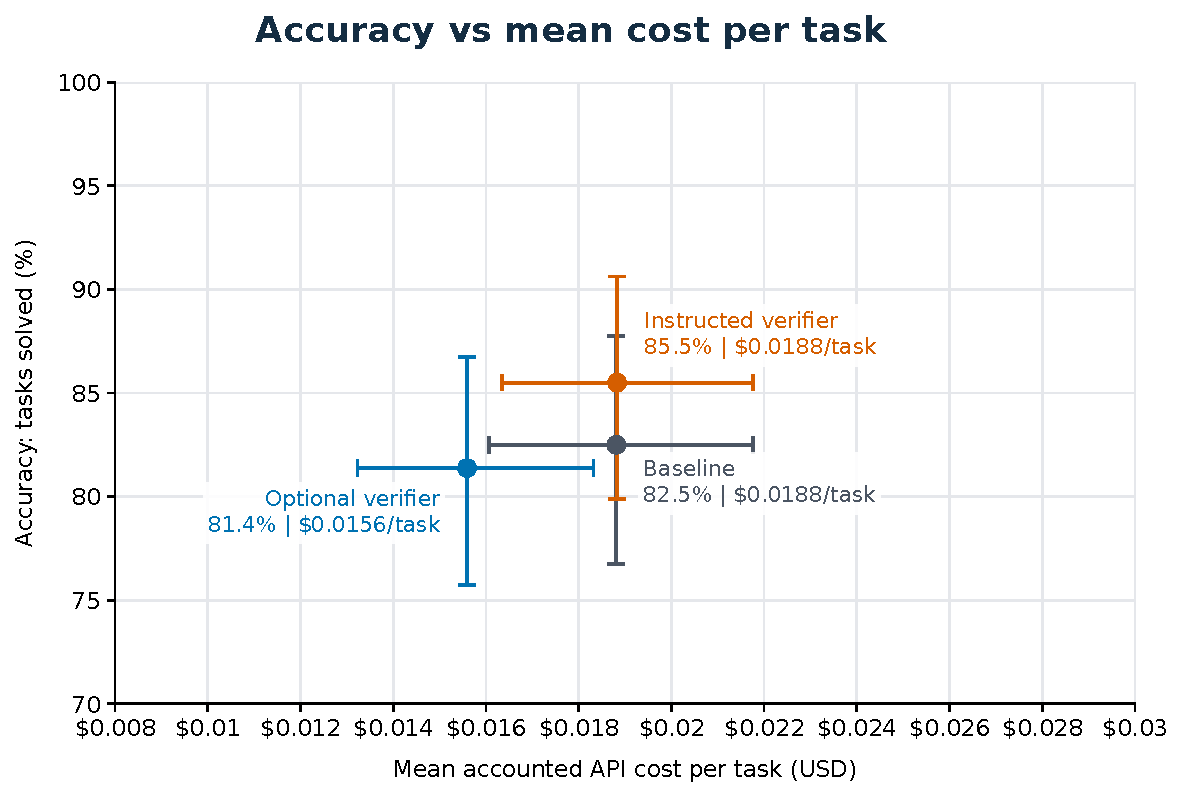
\includegraphics[width=0.73\linewidth]{accuracy-vs-cost-selected-attempts.pdf}
\captionof{figure}{Pooled accuracy versus mean API cost per evaluation. Error bars are marginal 95\% family-bootstrap intervals.}\label{fig:accuracy-cost}
\end{center}

Compared with baseline, the optional verifier scored 0.25 percentage points higher in the 2000--2399 band and 2.50 points lower in the 2400--3500 band. The instructed verifier scored 2.50 and 3.50 points higher than baseline in those bands, respectively. Each cell summarizes 400 evaluations.

\begin{center}
\small
\captionof{table}{Accuracy by Codeforces rating band.}\label{tab:rating}
\begin{tabular}{@{}lrrr@{}}
\toprule
Codeforces rating & Baseline & Optional verifier & Instructed verifier \\
\midrule
2000--2399 & 91.50\% & 91.75\% & \textbf{94.00\%} \\
2400--3500 & 73.50\% & 71.00\% & \textbf{77.00\%} \\
\bottomrule
\end{tabular}
\end{center}

In the instructed verifier condition, the agent invoked CrossHair in 639 of 800 runs. The logs recorded 1,016 \texttt{verify} calls across 1,015 shell actions. The audit recorded 1,141 outcome labels across four groups: 382 confirmations, 150 counterexamples, 436 inconclusive results, and 173 reports of unsupported constructs or missing checkable functions. The inconclusive group includes errors, timeouts, and actions without a clear diagnostic. A single shell action could contribute several labels.

The agent subsequently edited \texttt{main.py} in 173 of 639 runs with verifier use, including 30 of 106 runs with a reported counterexample.

\section{Limitations \& Threats to Validity}
The experiment evaluated a single model and verifier in one programming language. The benchmark included 100 distinct tasks, which limited the precision of the estimated differences in accuracy. Because the tasks are public, some may have appeared in the model's training data.

\newpage

\section{Conclusion}
Providing optional access to CrossHair resulted in zero invocations across 800 runs. With explicit verification instructions, the agent used CrossHair in 639 of 800 runs. Unsupported constructs, missing checkable functions, and inconclusive results still limited the feedback available to the agent.

Relative to baseline, accuracy was 1.13 percentage points lower with optional access and 3.00 points higher with instructed verification. Mean API cost in the instructed condition was only 0.09\% higher than baseline. The largest observed gain was 3.50 percentage points on Codeforces tasks rated 2400--3500. Both paired 97.5\% confidence intervals included zero and were compatible with an increase or a decrease in accuracy. The experiment therefore leaves H1 and H2 unresolved.

The observed gain provides a preliminary signal worth testing on a larger benchmark and across more experimental configurations, subject to available computing resources and funding for API usage.

\section{References}
\begin{enumerate}
\setlength{\itemsep}{4pt}
\item\label{ref:crosshair} CrossHair. \emph{Contracts and symbolic execution.} \href{https://crosshair.readthedocs.io/en/latest/contracts.html}{Documentation.}
\item\label{ref:mini} SWE-agent project. \emph{mini-SWE-agent.} \href{https://github.com/SWE-agent/mini-swe-agent}{Repository.}
\item\label{ref:humaneval} JetBrains. \emph{Kotlin HumanEval.} \href{https://huggingface.co/datasets/JetBrains/Kotlin_HumanEval}{Dataset.}
\item\label{ref:jormungandr} Jormungandr. \emph{Kotlin formal verification plugin.} \href{https://github.com/korrektness/jormungandr}{Repository.}
\item\label{ref:codecontests} Y. Li et al. \emph{Competition-level code generation with AlphaCode.} Science, 2022. \href{https://doi.org/10.1126/science.abq1158}{Paper.} \href{https://huggingface.co/datasets/deepmind/code_contests/tree/802411c3010cb00d1b05bad57ca77365a3c699d6}{CodeContests dataset snapshot.}
\item\label{ref:project} Project materials. \href{https://github.com/dimativator/plsd-verifier-project/tree/3e0232b9458f0681853c1f4cbed76878b6ab2abe}{Benchmark repository.} \href{https://github.com/dimativator/plsd-verifier-project/pull/1}{Main study pull request.}
\end{enumerate}

\section{Appendix}
\textbf{Reproduction.} Use Bash and Python~3.12 or later. Check out the pull request branch and run the commands from the repository root.

{\small
\begin{verbatim}
git clone https://github.com/dimativator/plsd-verifier-project.git
cd plsd-verifier-project
git fetch origin refs/pull/1/head
git checkout --detach FETCH_HEAD

python -m pip install -e ".[report]"
python -m zipfile -e studies/codeforces-20261124/data.zip runs/study
python -m experiments.three_arm_analysis --phase main \
  --results runs/study/combined-results.json \
  --expected runs/study/combined-expected.json \
  --output runs/analysis.json
python studies/codeforces-20261124/selected-attempts/rebuild-selected-attempts-plot.py \
  --study runs/study --output runs/accuracy-vs-cost-selected-attempts.pdf \
  > runs/selected-attempt-costs.json
\end{verbatim}
}

The commands reproduce the paired accuracy comparisons, cost summary, and figure from the archived outcomes.
\end{document}
